\documentclass[a4paper,fontsize=10pt,twoside,DIV15,BCOR12mm,headinclude=true,footinclude=false,pagesize,bibtotoc]{scrbook}


\usepackage[utf8]{inputenc}
\usepackage[T1]{fontenc}

\usepackage{pslatex} % -- times instead of computer modern
\usepackage[scaled=.84]{beramono} % a sane monospace font
%\usepackage{microtype}

\usepackage{url}
\usepackage{booktabs}
\usepackage{graphicx}
\usepackage{textcomp}
\usepackage{xspace}
\usepackage[usenames,dvipsnames,table]{xcolor}
\usepackage{colortbl}
\usepackage{multicol}
\usepackage{rotating}
\usepackage{subfig}
\usepackage{ulem}
\usepackage{enumerate}
\usepackage{fancyvrb}
\usepackage{framed}

% Doxygen includes
\usepackage{calc}
%\usepackage{../c_doc/latex/doxygen}
\usepackage{makeidx}
\usepackage{multirow}

% avoid clubs and widows
\clubpenalty=10000
\widowpenalty=10000

% tweak float placement
%% \renewcommand{\textfraction}{.15}
\renewcommand{\topfraction}{.75}
%% \renewcommand{\bottomfraction}{.7}
\renewcommand{\floatpagefraction}{.75}
%% \renewcommand{\dbltopfraction}{.66}
%% \renewcommand{\dblfloatpagefraction}{.66}
\setcounter{topnumber}{4}
%% \setcounter{bottomnumber}{4}
%% \setcounter{totalnumber}{16}
%% \setcounter{dbltopnumber}{4}

\newcommand{\code}[1]{{\texttt{#1}}}
\newcommand{\codefoot}[1]{{\textsf{#1}}}
\def\figref#1{Figure~\ref{fig:#1}}

% ulem package, otherwise emphasized text becomes underlined
\normalem


\newcommand{\todo}[1]{{\emph{TODO: #1}}}
%\renewcommand{\todo}[1]{}
\newcommand{\nopublish}[1]{}

%
% generic command to comment something
%
\newcommand{\ncomment}[3]{

\textsf{\textbf{#1}} {\color{#3}#2}}

%
% commentators
%
\newcommand{\wolf}[1]{\ncomment{Wolfgang}{#1}{OliveGreen}}
\newcommand{\martin}[1]{\ncomment{Martin}{#1}{Blue}}
\newcommand{\rasmus}[1]{\ncomment{Rasmus}{#1}{Mahogany}}

% uncomment to get rid of comments
\renewcommand{\wolf}[1]{}
\renewcommand{\martin}[1]{}
\renewcommand{\rasmus}[1]{}

%
% custom colors
%
\definecolor{lightgray}{gray}{0.8}
\definecolor{gray}{gray}{0.5}

\usepackage{listings}

% general style for listings
\lstset{basicstyle=\ttfamily,keywordstyle=\ttfamily,showstringspaces=false,language=C}

\usepackage[endianness=big]{bytefield}

% long immediate in second slot
\newcommand{\lconst}{\texttt{const}_{32}}
% short immediate in ALU instruction
\newcommand{\sconst}{\texttt{Constant}_{12}}
% constant in Rs2 field
\newcommand{\rconst}{\texttt{Constant}_{5}}

% SH: to be used in text mode .. maybe we should change this to math mode?
\newcommand{\XOR}{\textasciicircum\xspace}
\newcommand{\OR}{\textbar\xspace}
\newcommand{\AND}{\&\xspace}
\newcommand{\NOT}{\texttildelow}
\newcommand{\shl}{\textless$\!$\textless\xspace}
\newcommand{\shr}{\textgreater$\!$\textgreater$\!$\textgreater\xspace}
\newcommand{\ashr}{\textgreater$\!$\textgreater\xspace}

\newcommand{\bitsunused}{\rule{\width}{\height}}
\newcommand{\bitssubclass}{\color{lightgray}\rule{\width}{\height}}

\usepackage{mdwlist}
\renewenvironment{description}%
{
\begin{basedescript}{
\desclabelstyle{\nextlinelabel}
\renewcommand{\makelabel}[1]{%
\parbox[b]{\textwidth}{\bfseries##1}%
}%
\desclabelwidth{2em}}}
{
\end{basedescript}
}

%
% allow click-able links
%
\usepackage[open]{bookmark}
\usepackage[all]{hypcap}

%
% hyperref setup (depends on bookmark/hyperref}
%
\hypersetup{
    pdftitle = {Argo programming exercise},
    pdfsubject = {Technical Report},
    colorlinks = {true},
    citecolor = {black},
    filecolor = {black},
    linkcolor = {black},
    urlcolor = {black},
    final
}

%
% document contents
%
\begin{document}

\title{The Argo software perspective}
\subtitle{A multicore programming exercise}

\author{Rasmus Bo S{\o}rensen \\ {\normalsize Updated by Luca Pezzarossa}}

\lowertitleback{Copyright \copyright{} 2017 Technical University of Denmark
  \medskip\\
  \begin{tabular}{lp{.8\textwidth}}
    \raisebox{-12pt}{
\includegraphics[height=18pt]{fig/cc_by_sa}} &
     This work is licensed under a Creative Commons Attribution-ShareAlike
     4.0 International License.
     \url{http://creativecommons.org/licenses/by-sa/4.0/}\\
  \end{tabular}
}

\frontmatter

\maketitle

\chapter{Preface}

This exercise manual is written for the course `02211 Advanced Computer Architecture' at the Technical University of Denmark,
but is intended as a stand-alone document for anybody interested in learning about multicore programming with the Argo Network-on-Chip.

This document is subject to continuous development along with the platform it describes.
In case you have suggestions for improvement or find that the text is unclear and needs to be elaborated, please write to \href{mailto:rboso@dtu.dk}{rboso@dtu.dk} or \href{mailto:lpez@dtu.dk}{lpez@dtu.dk}.
The latest version of this document is contained as LaTeX source in the Patmos repository in directory
\code{patmos/doc} and can be built with \code{make noc}.

\nopublish{
\section*{Acknowledgment}

}

\tableofcontents

%\begingroup
%\let\cleardoublepage\clearpage
%\listoffigures
%\listoftables
%\lstlistoflistings
%\endgroup

\mainmatter

\chapter{Introduction}

This document presents the background required to write a multicore program utilizing the Argo NoC~\cite{t-crest:argo:tvlsi2015} for intercore communication in the T-CREST plaform~\cite{t-crest:2015}.
The exercises should give the reader a good understanding of how the Argo NoC can be utilized in a multicore application.
The reader will get experience in how to write a multicore application that uses message passing.
In the exercises, we assume that the reader is familiar with the C programming language and multi-threaded programming in general.
Furthermore, we assume that the reader has already run a single core application on a Patmos processor in an FPGA, refer to the Patmos handbook~\cite{patmos:handbook} for details on the Patmos processor.

An example of the multicore platform is shown in Fig.~\ref{fig:mc-patmos}. Core $P_0$ is referred to as the master core, and the rest of the cores are referred to as slave cores. The reason that $P_0$ is the master core is that when an application is downloaded to the platform, the application starts executing \code{main()} on the master core; also the serial console  is connected to the master core. All cores are connected to the shared external memory, but the bandwidth towards the external memory is quite low.
Therefore, the programmer should utilize the NoC as much as possible for core-to-core communication.
\begin{figure}[h]
\centering
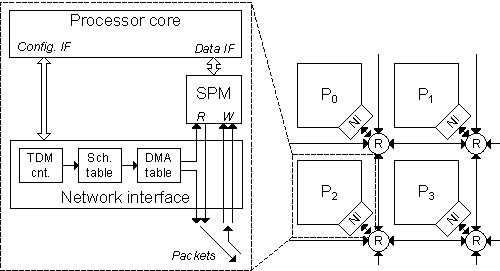
\includegraphics[width=0.9\textwidth]{fig/MultiCore.pdf}
\caption{The Patmos multicore platform with the Argo NoC for intercore communication.
The core with id 0 is referred to as the master core, and the rest of the cores are referred to as the slave cores.}
\label{fig:mc-patmos}
\end{figure}

Chapter~\ref{chap:arch} presents the architecture of the Argo Network-on-Chip.
Chapter~\ref{chap:api} describes the programming interface of the multicore platform, including the thread library and the high-level message passing.
Chapter~\ref{chap:exercise} contains the practical exercises to give the reader a practical introduction to the platform.
Finally, Appendix~\ref{apx:build} describes the practical aspects of loading the program into the platform running in an FPGA.
%Appendix~\ref{apx:api} contains the Doxygen documentation of the C libraries.


\chapter{The Architecture of Argo}
\label{chap:arch}
The Argo network-on-chip (NoC) is a time-predictable core-to-core interconnect. Argo can provide communication channels that have a guaranteed minimum bandwidth and maximum latency.
Argo uses direct memory access (DMA) controllers to perform write transactions through the NoC that is interleaved with the TDM schedule.
When Argo performs a write transaction through the NoC, it moves a block of data from the local scratchpad memory (SPM) to the SPM of another core in the network.


The guarantees on bandwidth and latency are enforced by a static time division multiplexing (TDM) schedule, where the network resources are allocated to communication channels.
A TDM schedule is generated by the Poseidon TDM scheduler, based on some bandwidth requirements that are given in XML format.
The statically allocated TDM schedule is loaded
into hardware tables in the network interface when the platform boots.
It is possible to reconfigure a new schedule at runtime with the reconfiguration capabilities of the Argo NoC, but since the reconfiguration capabilities are not needed for these exercises, they are not described in this document.
In these exercises, we assume the default all-to-all schedule where all cores have communication channels to all other cores.

Figure~\ref{fig:argo-arch} shows the architecture of the Argo NoC.
\begin{figure}[b!]
\centering
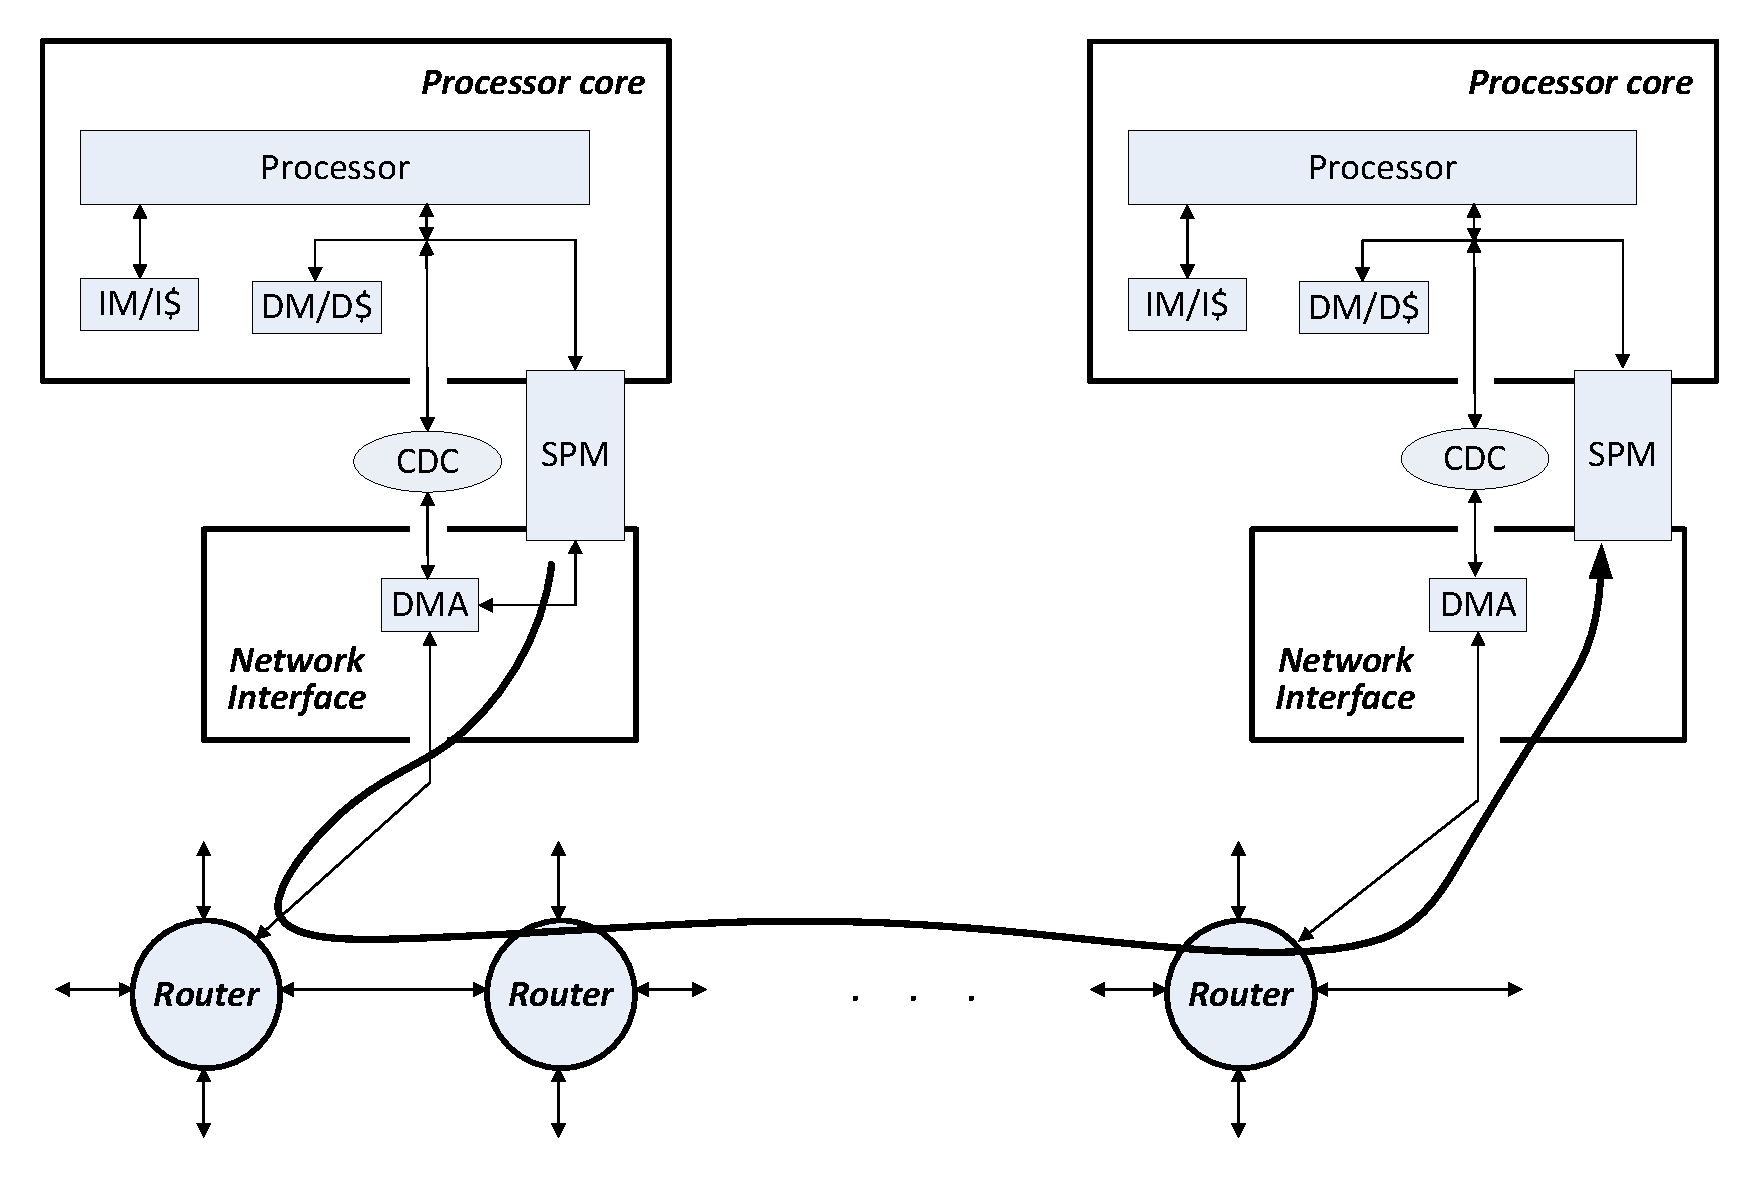
\includegraphics[width=\textwidth]{fig/argo-arch.pdf}
\caption{The Argo architecture from a software perspective.
A DMA write transaction moves the specified block of data from the
communication SPM of the processor on the left to the specified
location in the communication SPM of the processor on the right.}
\label{fig:argo-arch}
\end{figure}
The DMA block in the figure contains a table of DMA entries,
each entry describes a DMA controller that can send to a remote processor.
Each DMA controller is paired with a communication channel when the network is configured. 
To transfer a block of data from a local SPM to a remote SPM, there are \ref{arch:list1}~steps:
\begin{enumerate}
\item Store the block of data in the local SPM
\item Through the network interface set up the DMA controller that is paired with the correct communication channel by:
  \begin{itemize}
  \item Writing the local address of the block of data and the remote address to which the block of data should be moved
  \item Writing the size of the block of data
  \item Setting the `active' bit in the DMA entry to 1
  \end{itemize}
\label{arch:list1}\end{enumerate}
After step~\ref{arch:list1} the DMA will start to transfer data in each TDM slot that is allocated to the specified communication channel.
When the DMA has transferred all packets through the network the `active' bit is reset by the NI for that DMA entry. The `active' bit can be pooled to wait for the DMA to finish.

Conflicts of reading and writing to the same addresses in the dual
ported SPMs has to be handled by software; there is no protection in hardware.


% % % % % % % % % % % % % % % % % % % % % % % % % % % % % % % % % % % % % % % %
\chapter{Application Programming Interface}
\label{chap:api}
This chapter describes the Argo application programming interface (API).
The Argo API is made up of three libraries, the thread library \code{libcorethread}, the NoC Driver library \code{libnoc}, and the message passing library \code{libmp}. In the following three sections, we give an overview of the three libraries.
%For detailed documentation refer to Appendix~\ref{apx:api}, which contains the Doxygen documentation of the three C libraries.

\section{Corethread Library}
\label{sec:cthread}
When an application starts executing on the platform, \code{main()} is executed only on the master core with core ID 0.
From the \code{main()} function the programmer can start the execution of a function on the slave cores using the functions in the \code{libcorethread} library.
The functions of the \code{libcorethread} library are:
\begin{description}
\item[\code{int corethread\_create( int core\_id, void(*start\_routine)(void *), void *arg ) )}]

The create function will start the execution of the \code{start\_routine} function on the core specified by \code{core\_id}, an argument can be given to the started function via the \code{arg} pointer. The start function should only be called by the master core during the initialization phase of the application.

\item[\code{void corethread\_exit( void * retval )}]

The exit function can be called in the \code{start\_routine} functions if they need to return a value to the master core.
The exit function should be called as the last thing before the return statement.

\item[\code{int corethread\_join( int core\_id, void ** retval )}]

The join function will join the program flow of the master core with the program flow of the core specified by \code{core\_id}, and the join function should only be called from the master core. The join function will point the \code{retval} pointer to the return value allocated by the thread on the slave core. Be aware, the return value should not be allocated on the stack of the slave core!

\end{description}


\section{NoC Driver}
The NoC driver \code{libnoc} provides direct access to the hardware functionality and only abstracts the low-level accesses to hardware registers away.
There are driver functions for initialization of the NoC and for setting up DMA transfers.
The \code{libnoc} library is linked together with the auto-generated c file from the Poseidon scheduler. The auto-generated c file contains the schedule data.
The initialization of the NoC is done automatically before the \code{main()} function starts executing, if the compiler sees that the application uses any functions from the NoC driver.
If the application requires direct control over data movement through the NoC the following functions can be used, but it is very advisable to use the message passing library presented in Section~\ref{sec:libmp} to reduce the amount of manual memory allocation.


\begin{description}
\item[\code{int noc\_dma\_done( unsigned dma\_id )}]

The done function is used to tell whether a local DMA transfer has finished.

\item[\code{int noc\_nbwrite( unsigned dma\_id, volatile void \_SPM *dst, volatile void \_SPM *src, size\_t size )}]

The nbwrite function is a non-blocking function for writing a block of data at the address \code{src} of size \code{size} to the core with the core id \code{dma\_id} and the remote address \code{dst}. The nbwrite function will fail if the DMA controller is still sending the previous block of data.

\item[\code{void noc\_write( unsigned dma\_id, volatile void \_SPM *dst, volatile void \_SPM *src, size\_t size )}]

The write function is calling the nbwrite in a while loop until it returns success.

\end{description}

\section{Message Passing Library}
\label{sec:libmp}

The \code{libmp} adds flow control, buffering and memory management on top of the \code{libnoc}.
\code{libmp} implements two different concepts of message passing, queuing message passing and sampling message passing.
Queuing message passing implements a first-in-first-out queue where all messages have to be consumed by the receiver.
Sampling message passing implements atomic updated of a sample value, this sample value can be read multiple times or not read at all before the next update.

To communicate from one core to another, each core must create a port of the same type, either sampling or queuing. There must be one source port and one sink port. Furthermore, the unique channel identifier for the two ports must be the same.


\begin{description}
\item[\code{void \_SPM * mp\_alloc( coreid\_t id, unsigned size )}]

The alloc function will allocate a block of memory of size
\code{size} in the SPM local to the core with the id \code{id}.
The alloc function can only be called from the master core executing \code{main()}
and once the memory block is allocated, it cannot be freed.
In the current version of the software, the alloc function will not
give an out of memory error, so the programmer should be aware
to not allocate more local memory than what is present.

\item[\code{qpd\_t * mp\_create\_qport( unsigned int chan\_id, direction\_t direction\_type, size\_t msg\_size, size\_t num\_buf)}]

The create\_qport function allocates the static buffer structures of a communication channel
and initializes the queuing port descriptor \code{qpd\_ptr}.
The communication channel is set up between the sending
core \code{sender} and the receiving core \code{receiver}.
The communication channel will transfer messages of size
\code{msg\_size} and buffer a number of \code{num\_buf} messages in the receiver SPM.

\item[\code{int mp\_nbsend( mpd\_t* mpd\_ptr )}]

The nbsend function checks if there is a free buffer in the receiver
and if the DMA controller for the given communication channel is free.
If both are free, it will set up the DMA to transfer the new block of data.
The nbsend function assumes that the user/application already
wrote the data to be sent to the \code{write\_buf} buffer.

\item[\code{void mp\_send( mpd\_t* mpd\_ptr )}]

The send function calls the nb\_send function in a loop until it returns success.

\item[\code{int mp\_nbrecv( mpd\_t* mpd\_ptr )}]

The nbrecv function checks if the next buffer, in the buffer queue,
has received a complete message.
If a message is received, it will move the \code{read\_buf} pointer
to the beginning of the message,
such that the user/application can read the received data.

\item[\code{void mp\_recv( mpd\_t* mpd\_ptr )}]

The recv function calls the nb\_recv function in a loop until it returns success.

\item[\code{int mp\_nback( mpd\_t* mpd\_ptr )}]

The nback function increment the number of messages that
has been acknowledged and sends the updated value to the 
sender core, if the send does not succeed the number
of acknowledged messages is decremented.

\item[\code{void mp\_ack( mpd\_t* mpd\_ptr )}]

The ack function calls the nb\_ack function in a loop until it returns success.

\item[\code{spd\_t * mp\_create\_sport(unsigned int chan\_id, direction\_t direction\_type, size\_t sample\_size)}]

The create\_sport function allocates the static buffer structures of a communication channel
and initializes the sampling port descriptor \code{spd\_ptr}.
The communication channel is set up between the writer
core and the reader core.
The communication channel will transfer messages of size
\code{sample\_size}.

\item[\code{int mp\_write(spd\_t * sport, volatile void \_SPM * sample)}]

The write function writes the sample to the specified sampling port.

\item[\code{int mp\_read(spd\_t * sport, volatile void \_SPM * sample)}]

The read function reads a sample from the specified sampling port and places the sample according to the sample pointer.

\item[\code{int mp\_init\_ports()}]

The init\_ports function initializes all the created ports. All ports shall be created in the initialization phase of the program, and all cores need to call the init\_ports function to initialize its local ports.

\end{description}

% % % % % % % % % % % % % % % % % % % % % % % % % % % % % % % % % % % % 

\chapter{Exercises}
\label{chap:exercise}

The following exercises are made to run on the default
9 core platform for the Altera DE2-115 board.
Please refer to the Appendix~\ref{apx:buildhw} for instructions on
how to build an up-to-date hardware platform.

\section{Circulating tokens}
By creating an application that mimics streaming behavior between a number of processors, this exercise will illustrate to the reader how the basics of message passing work on Argo.
In this exercise, we will make an application that circulates a number of tokens in a ring of 8 slave processors.
The number of tokens should be configurable, but always less than the number of processors.
Each of the processors in the ring shall repeatedly execute the following \ref{list:ex1:num1}~steps:

\begin{framed}
\begin{enumerate}
\item Receive a token from the previous processor

\item Turn on the processor LED to indicate that the token is being processed

\item Wait for a random amount of time in the interval [100 ms; 1 s]
\label{list:step_rand}
\item Send the token to the next processor, when the send is complete Turn off the processor LED to indicate the token has been processed

\label{list:ex1:num1}\end{enumerate}
\end{framed}

\noindent Looking at the LEDs when the application runs,
the reader should see tokens move from one LED to the other.
This behavior should be easy to observe with only a few tokens.
This exercise is split into \ref{list:ex1:num2}~tasks:
\begin{framed}
\begin{enumerate}
\item Create a function that blinks an LED and create a thread on each slave core that executes the blink function
\item Extend the blink function to turn the LED on and off at random times
\item Extend the blink function to receive a message from the previous core in the ring and send a message to the next core in the ring
\item Change the blink function such that it sends the random seed value along with the token
\label{list:ex1:num2}\end{enumerate}
\end{framed}

\noindent In each task you should verify that your program is working as expected by compiling and downloading it to the platform.
Figure~\ref{fig:header} shows the libraries to include in your program and the definition of the NoC master core as core 0.
Moreover, it shows some useful functions to get information related to the multicore platform.

\begin{figure}
\begin{Verbatim}[xleftmargin=1cm,xrightmargin=1cm,frame=single,framesep=3mm]
const int NOC_MASTER = 0;
#include <stdio.h>
#include <string.h>
#include <stdlib.h>
#include <machine/patmos.h>
#include "libcorethread/corethread.h"
#include "libmp/mp.h"

get_cpucnt(); // returns the number of cores
get_cpuid(); // returns the core ID
\end{Verbatim}
\caption{\label{fig:header}Libraries to include, definition of the NoC master, and some useful functions.}
\end{figure}

\subsection{Task 1}
In this task, you should create a function that blinks the LED and execute the function on the slave processors.
The frequency of blinking the LED should be in the order of 1~-~10~Hz so that it is visible to the eye.
Figure~\ref{fig:ctrl_led} shows an example of how to blink an LED, where the frequency of the blinking is set through a parameter of the blinking function.
To turn the LED on and off, write a 1 and 0, respectively to the hardware address of the LED. 

\begin{figure}
\begin{Verbatim}[xleftmargin=1cm,xrightmargin=1cm,frame=single,framesep=3mm]
//blink function, period=0 -> ~10Hz, period=255 -> ~1Hz
void blink(int period) {
    // The hardware address of the LED
    #define LED ( *( ( volatile _IODEV unsigned * ) 0xF0090000 ) )

    for (;;)
    {
        for (int i=400000+14117*period; i!=0; --i){LED = 1;}
        for (int i=400000+14117*period; i!=0; --i){LED = 0;}
    }
    return;
}
\end{Verbatim}
\caption{\label{fig:ctrl_led}An example of a function to blink a LED with the period as parameter.}
\end{figure}

To execute the \code{blink()} function on the slave core there is an example of
how to call the \code{corethread\_create()} function in Figure~\ref{fig:corethread}.
Section~\ref{sec:cthread} explains in further detail, how corethreads are started
on slave processors and how a parameter can be passed to the function.

\begin{figure}
\begin{Verbatim}[xleftmargin=1cm,xrightmargin=1cm,frame=single,framesep=3mm]
void loop(void* arg) {
  int num_tokens = *((int*)arg);
  /*
    Write code in the slave loop
  */
}

int main() {
  int worker_id = 1; // The core ID
  int parameter = 42;
  corethread_create( worker_id, &loop, (void*) &parameter );  

  int* res;
  corethread_join( worker_id, &res ); // No return value is returned

  return *res;  
}
\end{Verbatim}
\caption{\label{fig:corethread}An example of how to create a corethread.}
\end{figure}

\paragraph*{Expected output}
The 8 LEDs on the board should all blink with the specified frequency.

\subsection{Task 2}
In task 2 you shall extend the blink function from task 1 to turn the LED on and off at random times.
We suggest to use the \code{rand\_r()} function to generate a random number,
\code{rand\_r()} takes a pointer to a seed value in order to generate a random number.
Do not use the \code{rand()} function as it is not thread-safe.
The seed value in each core should be different; otherwise, all cores have the
same sequence of pseudo-random numbers.

Use the lower bits of the random number to generate a number on the desired range.
The \code{get\_cpu\_usecs()} function returns the value of the microsecond counter as an \code{unsigned long long}. 

\paragraph*{Expected output}
The 8 LEDs should now independently blink with random varying frequencies.

\subsection{Task 3}
In this task, you will start sending messages in order to move the tokens between the slave cores.
The use of the message passing function is described in Section~\ref{sec:libmp}.
The initialization of the message passing channels shall be done in the slave threads, and before messages can be sent or received, each slave needs to initialize the message passing channels with the \code{mp\_chan\_init()} function.
Figure~\ref{fig:open_channel} shows an example of how slave core 1 opens a source port (to send) towards core 2 and how slave core 2 opens a sink port (to receive) form core 1, creating a communication channel identified by the id 1 (first parameter in the function).

\paragraph*{Expected output}
It should now be observable that the tokens move between cores.

\begin{figure}
\begin{Verbatim}[xleftmargin=1cm,xrightmargin=1cm,frame=single,framesep=3mm]
#define MP_CHAN_NUM_BUF 2
#define MP_CHAN_BUF_SIZE 40

...

// Slave function running on core 1
void slave1(void* param) {
    // Create the port for channel 1
    qpd_t * chan1 = mp_create_qport(1, SOURCE, 
    MP_CHAN_BUF_SIZE, MP_CHAN_NUM_BUF);
    mp_init_ports();

    // Do something
    return;
}

// Slave function running on core 2
void slave2(void* param) {
    // Create the port for channel 1
    qpd_t * chan1 = mp_create_qport(1, SINK, 
    MP_CHAN_BUF_SIZE, MP_CHAN_NUM_BUF);
    mp_init_ports();

    // Do something
    return;
}
\end{Verbatim}
\caption{\label{fig:open_channel}An example of how to create a communication channel.}
\end{figure}


\subsection{Task 4}
For the sake of the example, you should now pair a seed value to each token.
To send the seed value along with the message, you need to write the seed value into
the \code{write\_buf} before sending the message, and read out the seed value from the \code{read\_buf}
after receiving a message.
Figure~\ref{fig:msg_data} shows an example of how to receive, send, acknowledge reception, read, and write message data.

\begin{figure}
\begin{Verbatim}[xleftmargin=1cm,xrightmargin=1cm,frame=single,framesep=3mm]
// Receiving, reading and acknowledge reception of 
// an unsigned integer value from the channel read buffer
mp_recv(chan,0);
seed = *(( volatile int _SPM * ) ( chan->read_buf )); 
mp_ack(chan,0);

// Writing an unsigned integer value to the channel 
// write buffer and sending it.
*( volatile int _SPM * ) ( chan->write_buf ) = seed; 
mp_send(chan,0);
\end{Verbatim}
\caption{\label{fig:msg_data}An example of how to receive, send, acknowledge reception, read, and write message data.}
\end{figure}

\paragraph*{Expected output}
It should now be observable that the tokens move between cores, like task 3 but with random intervals.

\subsection{Extensions}
If you have more time left or just can not get enough of programming message passing applications, you can extend your application  in several ways:
\begin{itemize}
\item Move the calculation of random numbers to core 0.
Core 0 shall act like a server replying with a new random number when it receives a message from any of the slave cores.
\item Create a mechanism that terminates the execution of the blink function on the slaves when the master is signaled to stop thought the terminal. 
\end{itemize}

\nopublish{

\section{Circulating tokens - WCET}

This exercise will show how to calculate the maximum worst case throughput of tokens.
The exercise comprise the following tasks:
\begin{itemize}
\item Compile with platin
\item 
\label{list:ex2:num1}\end{itemize}

\section{Next exercise}

Ideas for other exercises:
\begin{itemize}
\item WCET analysis of the circulating tokens
  \begin{itemize}
  \item Worst case throughput of tokens
  \item Worst case latency of a token through two processors
  \end{itemize}
\item Health monitoring 
\item I/O server
\end{itemize}

}
%%%%%%%%%%%%%%%%%%%%%%%%%%%%%%%%%%%%%%%%%%%%%%%%%%%%%%%%%%%%
% The start of the appendix
\appendix

%%%%%%%%%%%%%%%%%%%%%%%%%%%%%%%%%%%%%%%%%%%%%%%%%%%%%%%%%%%%%%%%%%%%%%%%%%%%%%
\chapter{Build And Execute Instructions}
\label{apx:build}

In this chapter, we present the details on how to 
build and configure the hardware platform and compile and execute 
a multicore program on the platform.

\section{Build and configure the hardware platform}
\label{apx:buildhw}

The Aegean framework generates a hardware description from an
XML description.
The default XML description for the Altera DE2-115 board with 9 cores
has an external shared memory and an Argo network-on-chip.
To build the platform run the following commands:
\begin{Verbatim}
cd ~/t-crest/aegean
make AEGEAN_PLATFORM=altde2-115-9core platform synth
\end{Verbatim}
The make command will generate a platform as described in the
\code{config/altde2-115-9core.xml} file.
When the platform description is generated, then it will be synthesised.
When the synthesis is finished the multicore platform can be
configured into the FPGA using the following commands:
\begin{Verbatim}
cd ~/t-crest
make -C aegean AEGEAN_PLATFORM=altde2-115-9core config
\end{Verbatim}

If you experience problems in building the multicore platform, you may need to update your T-CREST repositories to the newest version and re-build the project with the following commands before re-executing the commands listed above:
\begin{Verbatim}
cd ~/t-crest/
./misc/gitall pull
cd ~/t-crest/argo/
git pull
cd ~/t-crest/
./misc/build.sh -c
\end{Verbatim}

If you still experience problems, please send an email to \textit{lpez@dtu.dk} (Luca Pezzarossa).

\section{Compile and execute a multicore program}
\label{apx:buildsw}

There is no difference between compiling a single core program and a multicore program.
Furthermore, a single core program can execute in a multicore
platform without any modifications.
To compile a multicore program, place it in the \code{patmos/c/} directory
and run the following commands:

\begin{Verbatim}
cd ~/t-crest
make -C patmos APP=${APP_NAME} comp
\end{Verbatim}

The \code{comp} target will compile the C program in the file \code{patmos/c/\$\{APP\_NAME\}.c}
and output an .elf file \code{patmos/tmp/\$\{APP\_NAME\}.elf}.
When compiling a program that includes either \code{``libmp/mp.h''} or \code{``libnoc/noc.h''},
the \code{nocinit.c}, generated by the Aegean framework, is included needed,
as this contains the configuration data for the Argo NoC.
To download the program to the configured FPGA, run the following commands:

\begin{Verbatim}
cd ~/t-crest
make -C patmos APP=${APP_NAME} download
\end{Verbatim}

The \code{download} target of the Makefile depends on the comp target,
therefore it is not necessary to execute the \code{comp} target before every download.
Also, it is not strictly necessary to configure the FPGA with the hardware
platform between each download of a program, but we advise you to do so.
This will ensure that the hardware platform is probably initialized
before you download a program.


% % % % % % % % % % % % % % % % % % % % % % % % % % % % % % % % % % % % % % % %

\bibliographystyle{abbrv}
%\bibliography{argobib.bib}
\bibliography{../html/t-crest.bib}

\end{document}